\documentclass[a4paper, oneside]{article}
\usepackage[utf8]{inputenc}
\usepackage[czech]{babel}
\usepackage{amsmath}
\usepackage{amssymb}
\usepackage{amsfonts}
\usepackage{graphicx}
\begin{document}
\author{Bc. František MACH, Ing. Pavel Karban, Ph.D.}
\date{\today}
\section{Agros2D - výpočet kapacity jiskřiště a indukčnosti dvojlinky}
V tomto díle se více zaměříme na samotné řešení (processing) problémů a ukážeme si základy práce s příkazy. Budeme řešit dva příklady a to výpočet kapacity jiskřiště a výpočet indukčnosti dvojvodičového kabelu.
\subsection{Obsah}
Úvod\\
Vypočet kapacity jiskřiště\\
 - Příprava problému\\
 - Řešení\\
Vypočet indukčnosti dvojlinky\\
 - Příprava problému\\
 - Řešení\\
 \subsection{Úvod}
Jak již bylo řečeno v minulém díle seriálu, Agros2D využívá pro řešení parciálních diferenciálních rovnic popisujcích rozložení řešeného pole knihovnu Hermes2D (http://hpfem.org/hermes2d), která je vývíjena v rámci hp-FEM Group (http://hpfem.org) do které se řadí Nevadská univerzita v Renu, Akademie věd České republiky a také Západočeská univerzita v Plzni.\\
Knihovna Hermes2D umožňuje řešit parciální diferenciální rovnice pomocí hp-FEM, která je obdobou klasické FEM (Finite Element Method). hp-FEM kombinuje změnu velikosti elementů (zjemnění řešené sítě) a změnu řádu polynomu, kterým je každý element proložen. Těmito změnami je zajištěna exponencielní konvergence výsledků. Pro provádění těchto změn využívá Hermes2D automatickou hp-adaptivitu (h-adaptivitu, p-adaptivitu), která se provádí na základě největších gradientů řešené veličiny.\\
Agros2D rozlišuje mezi počáteční a řešenou sítí. Počáteční síť může být velmi hrubá. Při řešení je pak upravena díky automatické adaptivitě změnou velikosti jednotlivých elementů. Toho lze dosáhnout jak ručním nastavením určité oblasti, celého problému nebo využitím již zmiňované automatické hp-adaptivity.\\
\subsection{Výpočet kapacity jiskřiště}
Jiskřiště je elektrické zařízení, které se využívá při měření a spínání vysokých a velmi vysokých napětí. Nejčastěji se skládá ze dvou elektrod, které mohou být provedeny v mnoha tvarech. Je možné se setkat s kulovými elektrodami, hroty, elektrodami deskovými a mnoha dalšími.\\
Princip činnosti jiskřiště je založen na přeskoku v plynném nebo kapalném prostředí. Tohoto přeskoku lze však dosáhnout až za hranicí přeskokového napětí a je tedy možné tohoto napětí využít pro spínání nebo právě měření. V tomto příkladu budeme řešit elektrostatické pole mezi hrotem a deskovou elektrodou jiskřiště a následně vypočteme celkovou kapacitu daného uspořádání, která je potřebná například k určení nabíjecích charakteristik.\\
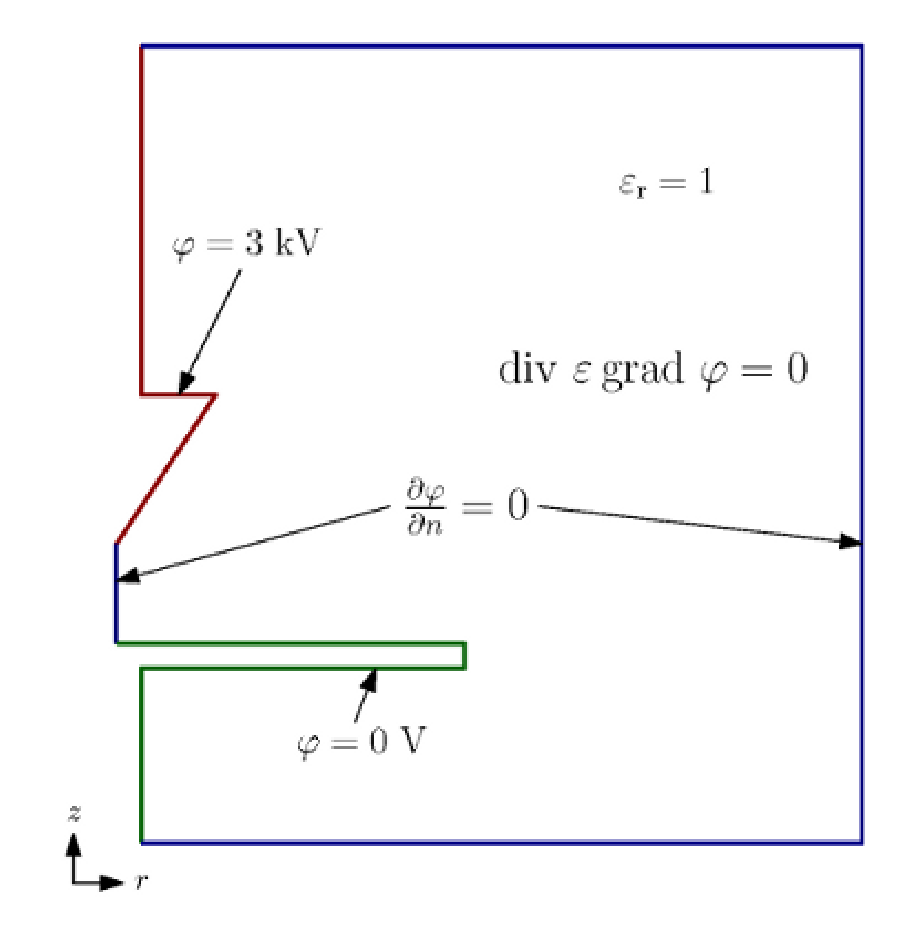
\includegraphics[width=6cm]{Matematicky_model_jiskriste.eps}\\
\subsection{Příprava problému}
Založíme nový problém. Jako typ řešeného pole zvolíme Elektrostatické pole a jako typ problému Osově symetrický. Vzhledem k povaze úlohy (velký gradient elektrického potenciálu na ostrých hranách hrotu) využijeme při řešení úlohy automatickou hp-adaptivitu, kterou vybereme v příslušném seznamu. Počet adaptivních kroků nastavíme na 10 a relativní chybu (relativní rozdíl výpočtu energetické normy v aktuálním a předchozím adaptivním kroku) na 5\%. Vzhledem k tomu, že využíváme automatickou adaptivitu, nastavíme počet zjemnění (parametr udávající počet zjemnění celé sítě) na nulu a řád polynomu (nejnižší použitý řád polynomu pro celý problém) na jedničku.\\
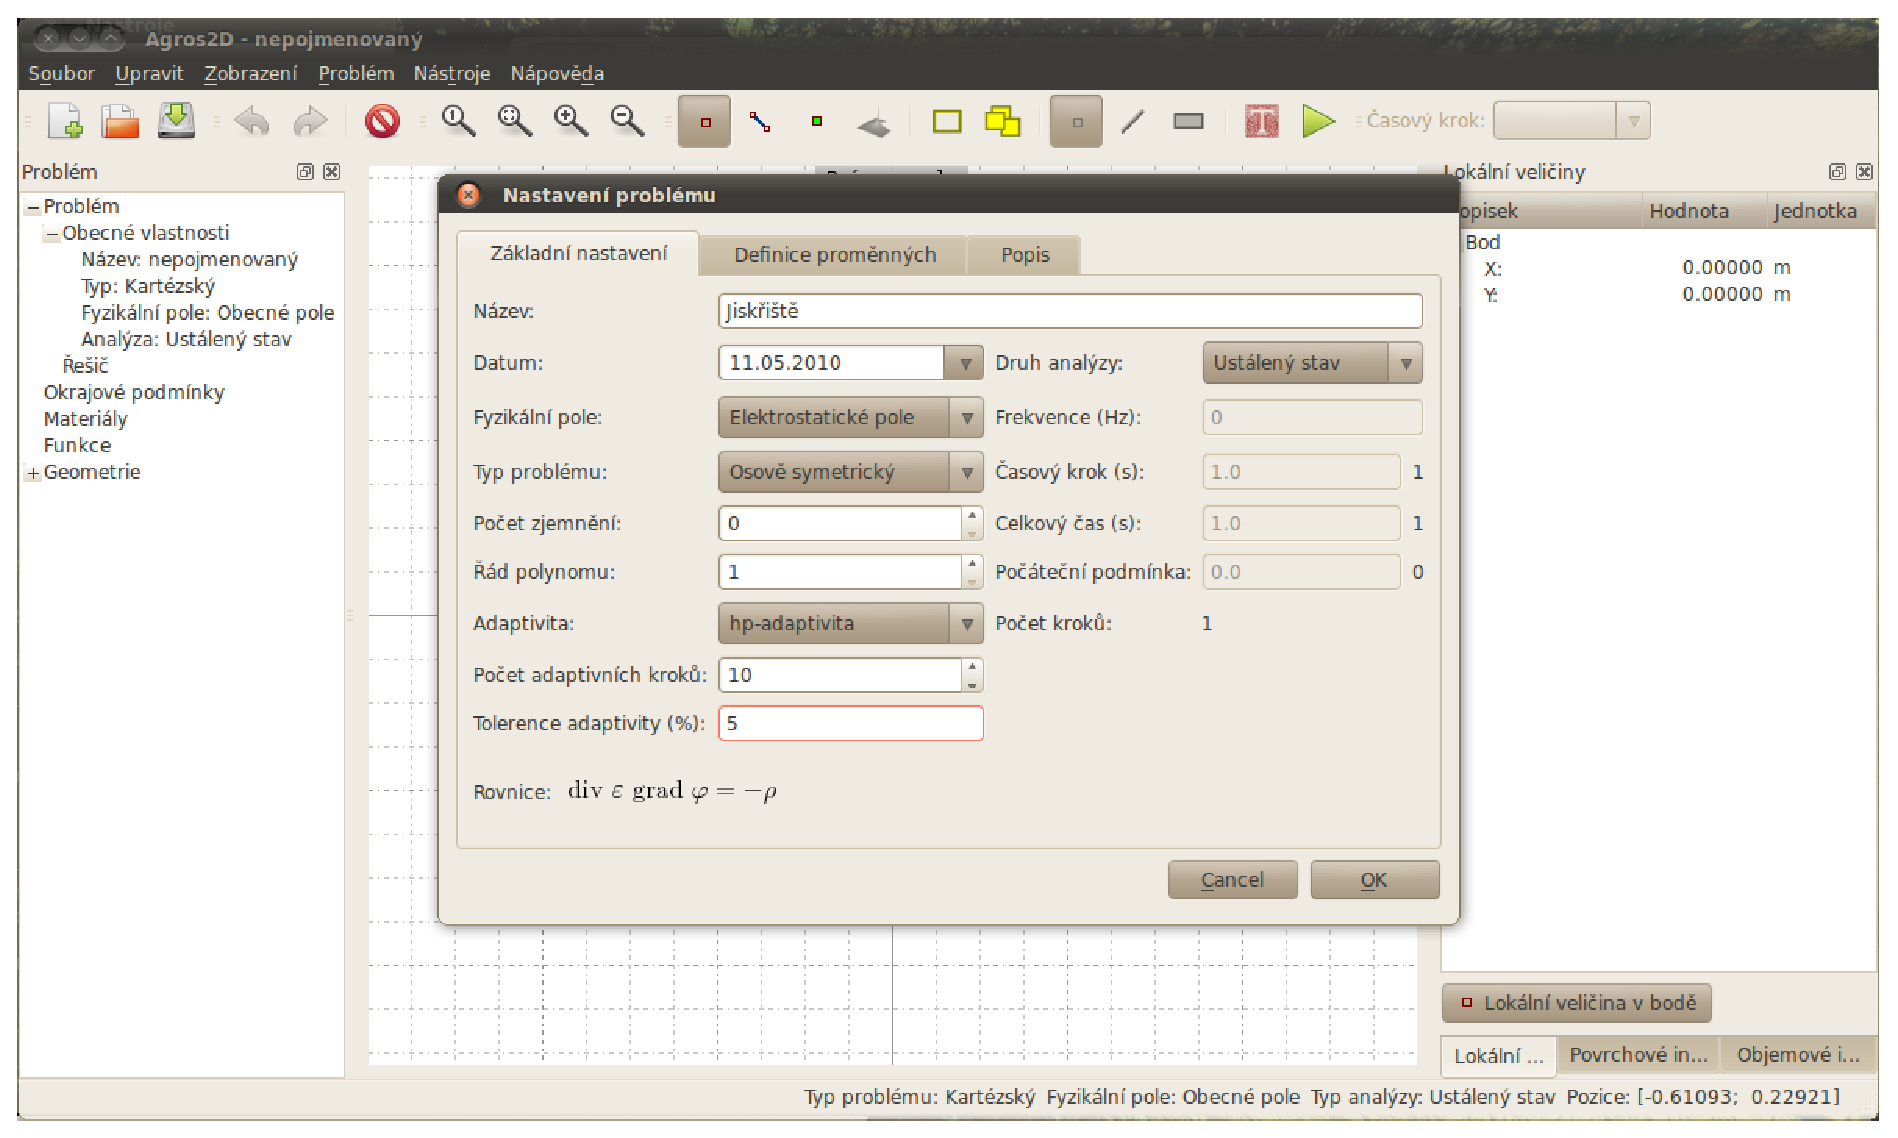
\includegraphics[width=12cm]{Nastaveni_problemu.eps}\\
Podle nákresu geometrie a níže uvedené tabulky přidáme postupně všechny potřebné body a následně je propojíme pomocí hran. Vznikne nám tak geometrie o jedné jediné ploše, která reprezentuje okolní prostředí jiskřiště. Do této plochy je nutné přidat značku plochy.\\
\begin{tabular}{|c|c|c|c|c|c|c|c|c|c|c|c|}
\hline
r(m) & 0 & 0.15 & 0.15 & 0 & 0 & 0.015 & 0 & 0 & 0 & 0.35 & 0.35\\
\hline
z(m) & 0 & 0 & 0.01 & 0.01 & 0.06 & 0.11 & 0.11 & 0.31 & -0.2 & 0.31 & -0.2\\
\hline 
\end{tabular} \\
Dále nadefinujeme okrajové podmínky. Řešený problém popisují čtyři okrajové podmínky, které respektují zdrojovou elektrodu, zemnící elektrodu, hranici symetrie a fiktivní hranici ohraničující řešenou oblast. Hranice zdrojové a zemnící elektrody (Hrot, Deska) popisuje Dirichletova okrajová podmínka a je na nich zadán elektrický potenciál. Pro hranu hrotu použijeme 3 kV a pro hranu desky 0 V. Hranice symetrie i fiktivní hranice jsou popsány Neumannovou okrajovou podmínkou a je na nich zadána derivace elektrického potenciálu ve směru vnější normály. Vzhledem k osové symetrii a nulové hodnotě normálové složky intenzity elektrického pole musí být tato derivace na obou hranicích (Symetrie, Fiktivní hranice) rovna nule.\\
Dále nadefinujeme potřebné materiály. V tomto příkladě to bude poměrně jednoduché, protože jediný materiál (Vzduch), který se v problému vyskytuje je okolní prostředí elektrod, kde budeme uvažovat vzduch. Ten má relativní permitivitu rovnou jedné. Nyní již stačí definované okrajové podmínky a materiály přiřadit. Na druhém obrázku níže je 3D náhled na geometrii řešeného problému.\\
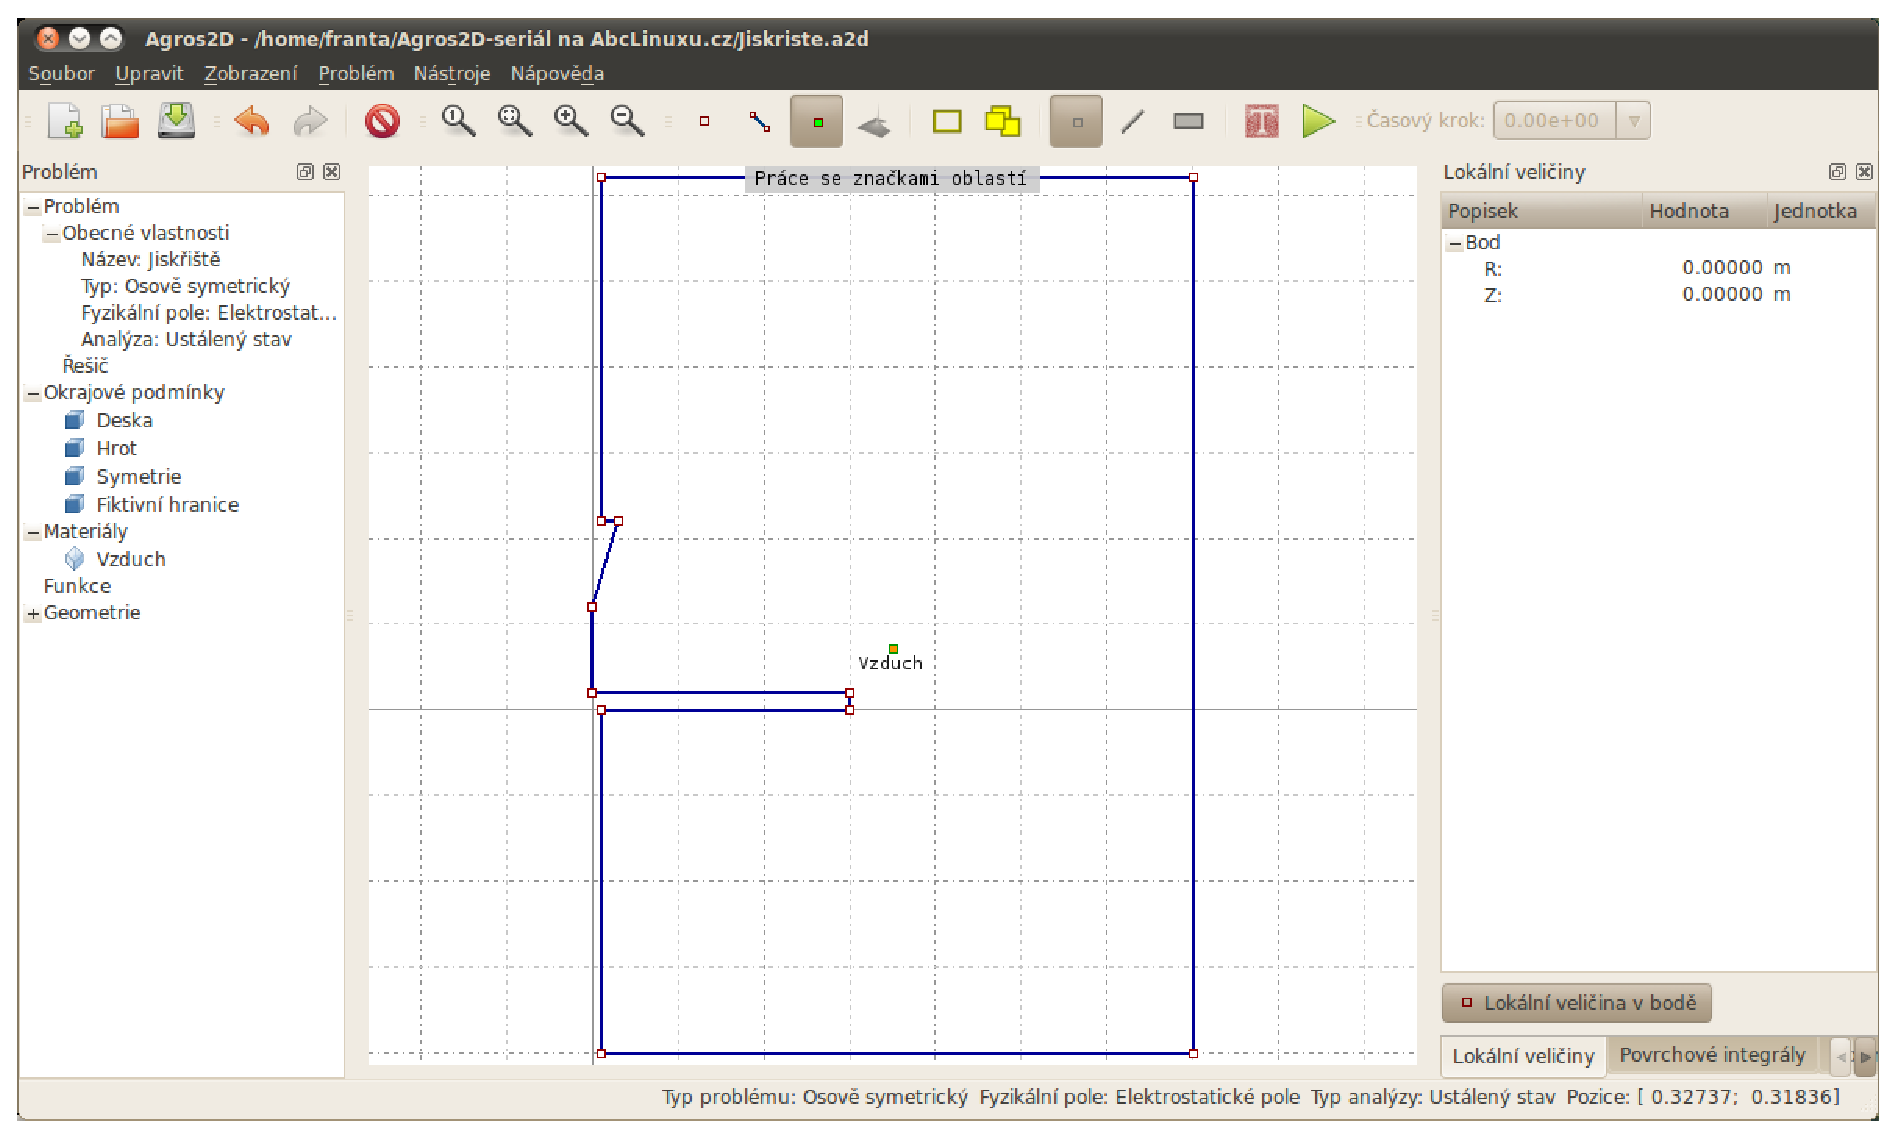
\includegraphics[width=5cm]{Geometrie_prvniho_problemu.eps}
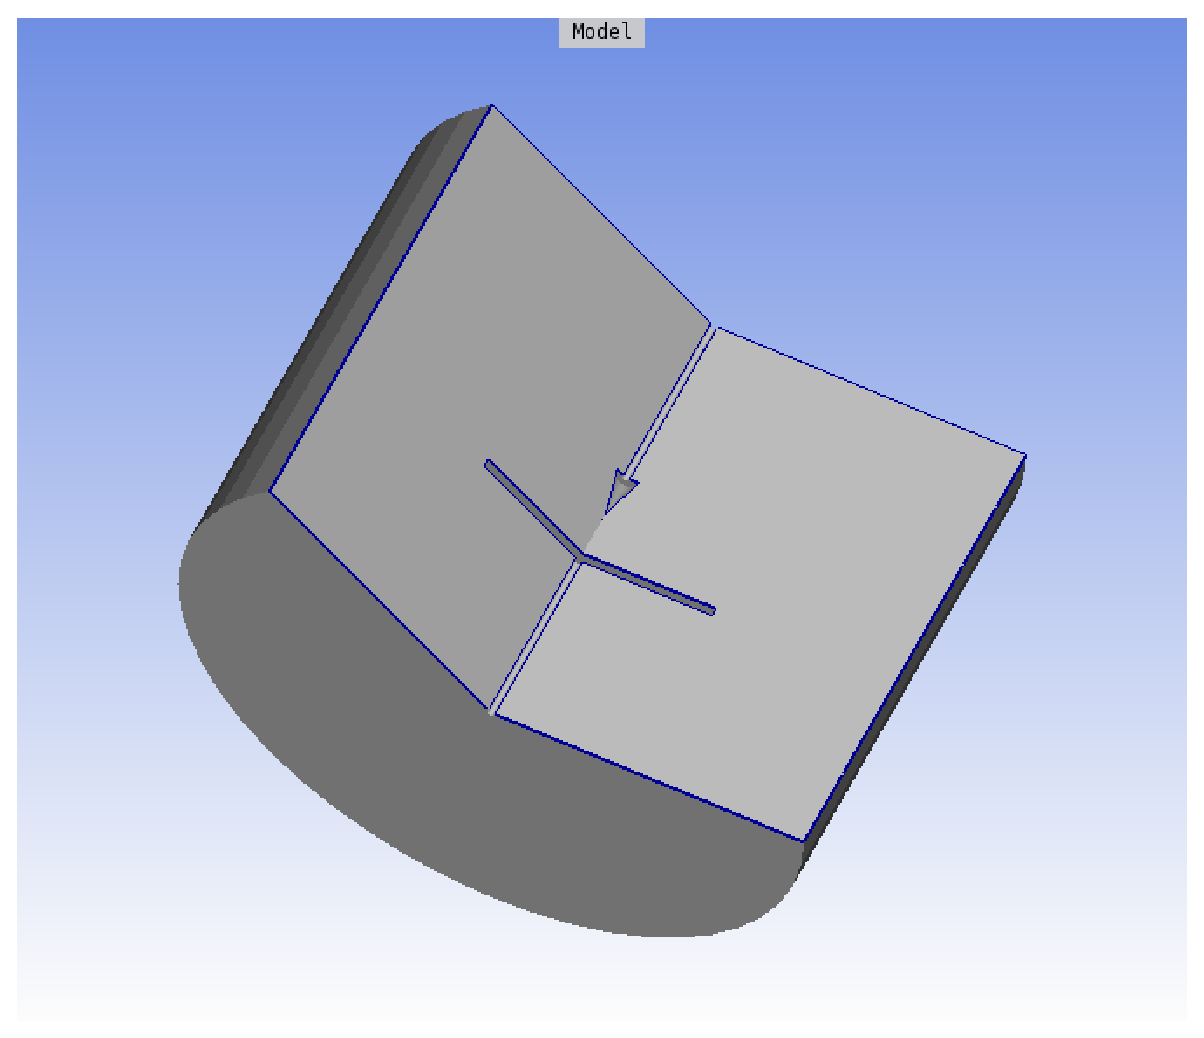
\includegraphics[width=5cm]{Model.eps}\\
\subsection{Řešení}
Nejprve problém diskretizujeme. Pokud vše proběhne v pořádku, můžeme přistoupit k samotnému řešení. Z výstupu řešiče je patrné, že relativní chyba výpočtu nedosáhla požadovaných 5\% a je tedy nutné zvýšit počet adaptivních kroků v dialogu Nastavení problému. Zkusíme tedy nastavit 20 adaptivních kroků a řešení zopakujeme. Tentokráte již relativní chyba dosáhla méně než 5\% a řešení můžeme považovat za dostatečně přesné. Ze zobrazení počáteční sítě, sítě řešené a řádu polynomu které si můžete navolit v dialogu Nastavení scény je patrné, že v okolí ostrých rohů elektrod a v prostoru mezi nimi došlo k automatickému zjemnění a využití různých řádů polynomů. U zobrazeného průběhu potenciálu mezi deskou a hrotem je patrný jeho strmý nárust a tedy i vysoká hodnota intenzity elektrického pole v těsné blízkosti hrotu.\\
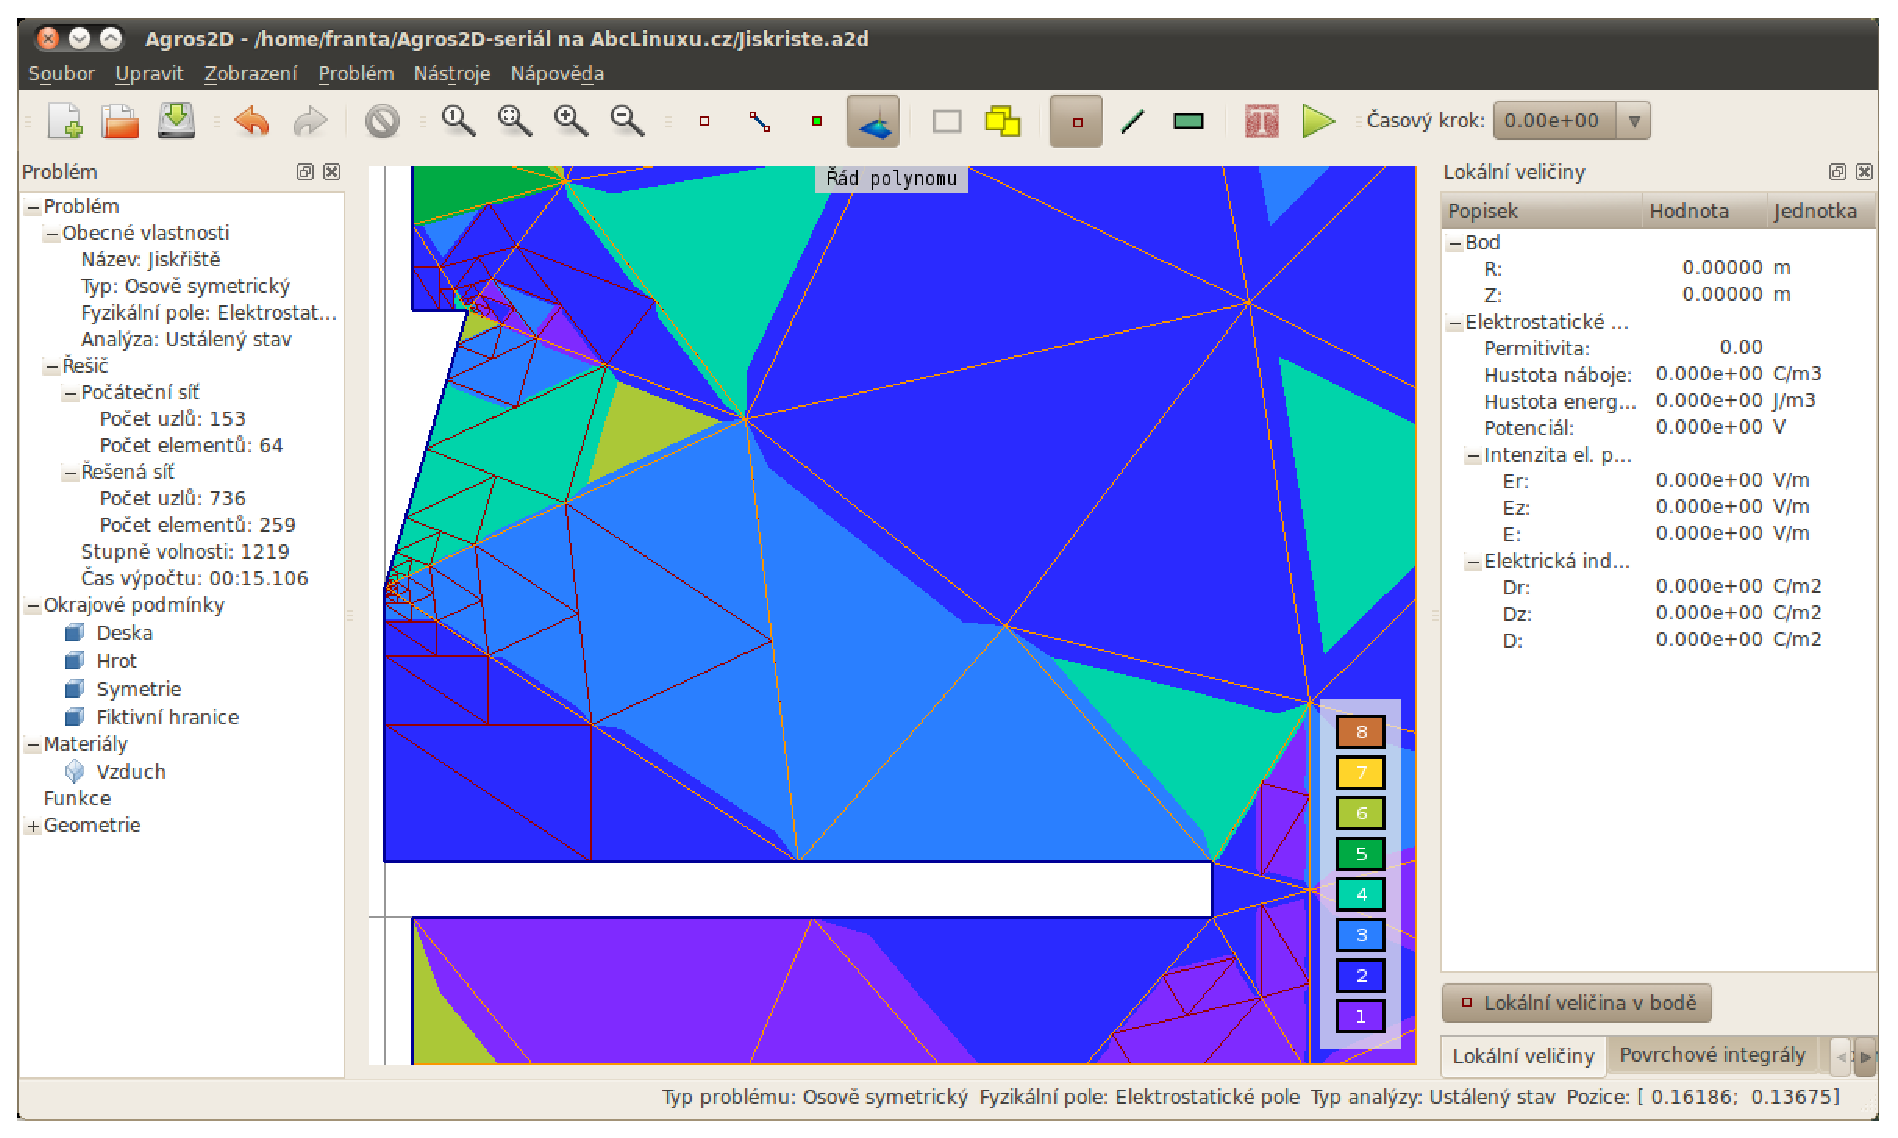
\includegraphics[width=6cm]{Sit_a_rad_polynomu.eps}
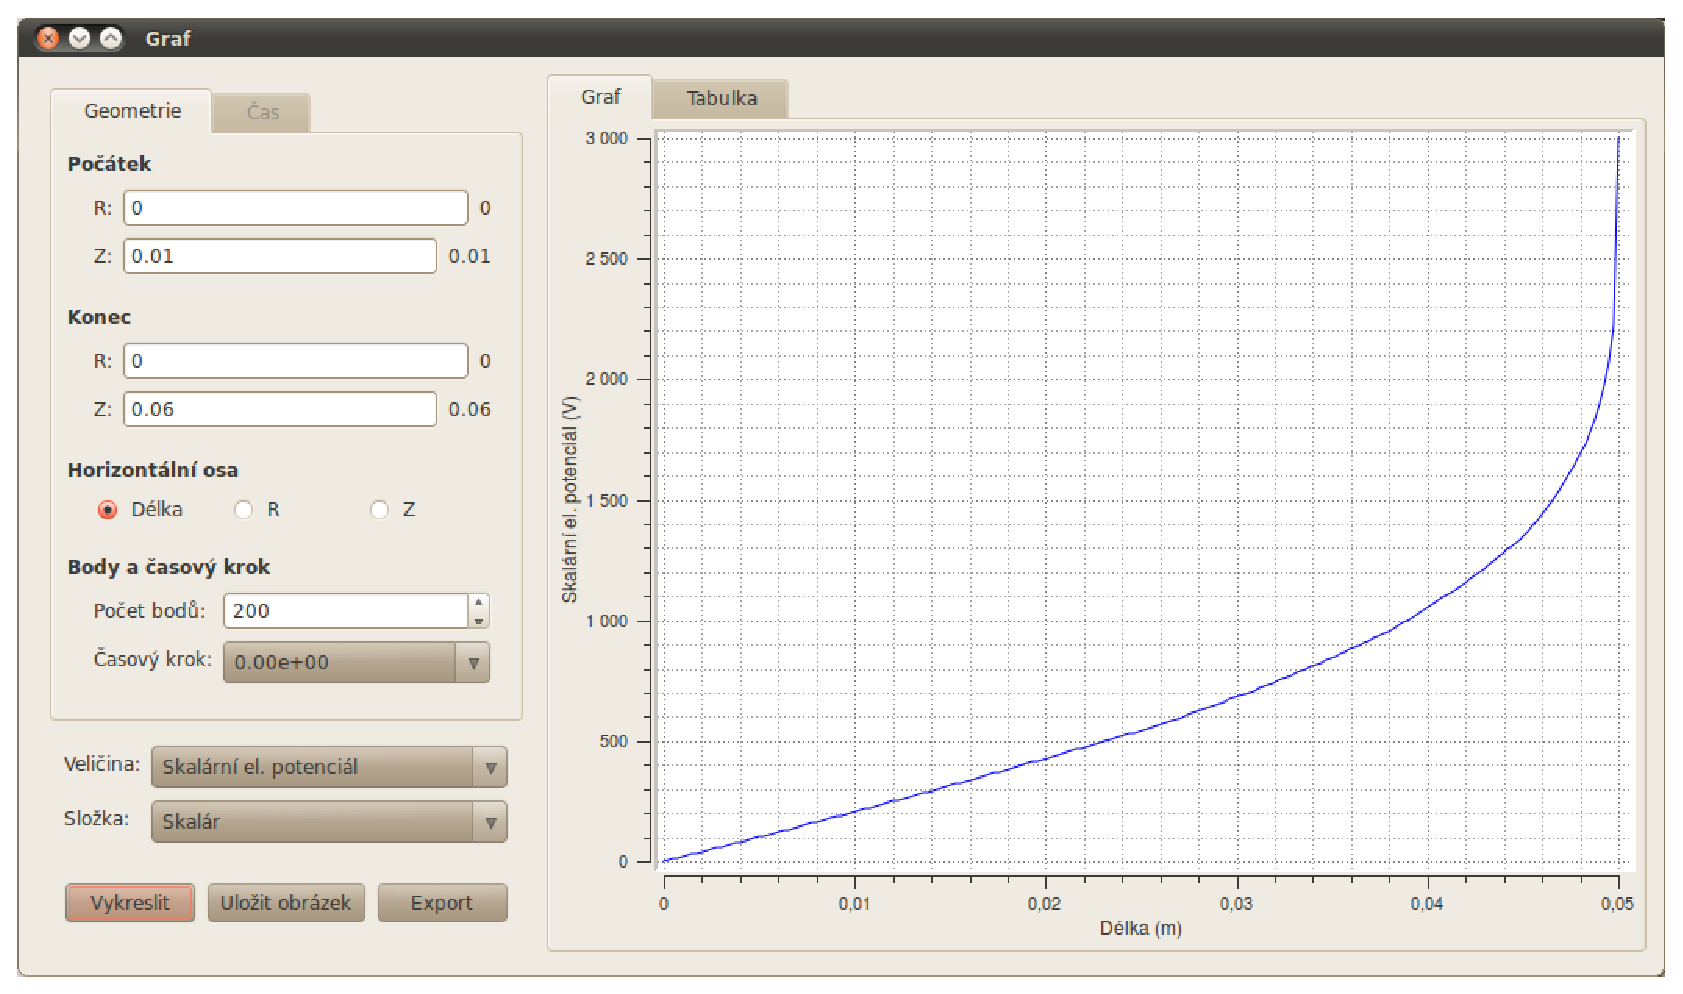
\includegraphics[width=6cm]{Graf.eps}\\		
Pro kontrolu správnosti řešení u elektrostatických problémů je výhodné využít zobrazení ekvipotenciál (čar spojující místa se stejným potenciálem) a vektorů intenzity elektrického pole, které si můžete opět nastavit v dialogu Nastavení scény. Je patrné, že vektory intenzity elektrického pole směřují vždy od hrotu k desce a ekvipotenciály respektují fyzikální realitu rozložení elektrického potenciálu mezi elektrodami.\\
Kapacitu jiskřiště lze spočítat dvěma způsoby. První z nich vychází z definice energie elektrostatického pole v lineárním prostředí a druhý z celkového náboje na jedné z elektrod, který je pro obě elektrody kvantitativně stejný a liší se pouze v polaritě. Využijeme první způsob a spočteme si tedy nejprve celkovou energii v oblasti vzduchu. Tato energie je rovna 171,2 mJ. Na základě vztahu $We = 0.5 CU^2$ lze tedy již vypočítat kapacitu mezi elektrodami. Tento výpočet můžeme provést přímo v terminálu Agros2D, který využívá skriptovacího jazyka Python. Pomocí položky Spustit příkaz... v menu Nástroje nebo klávesové zkratky Alt+C si otevřeme terminál a využijeme pro výpočet příkaz uvedený níže. Kapacita jiskřiště je rovna 11,413 pF. Na druhém obrázku níže je vykresleno rozložení elektrického potenciálu v prostoru jiskřiště.\\
print(2*1.712e-05/3e6)\\
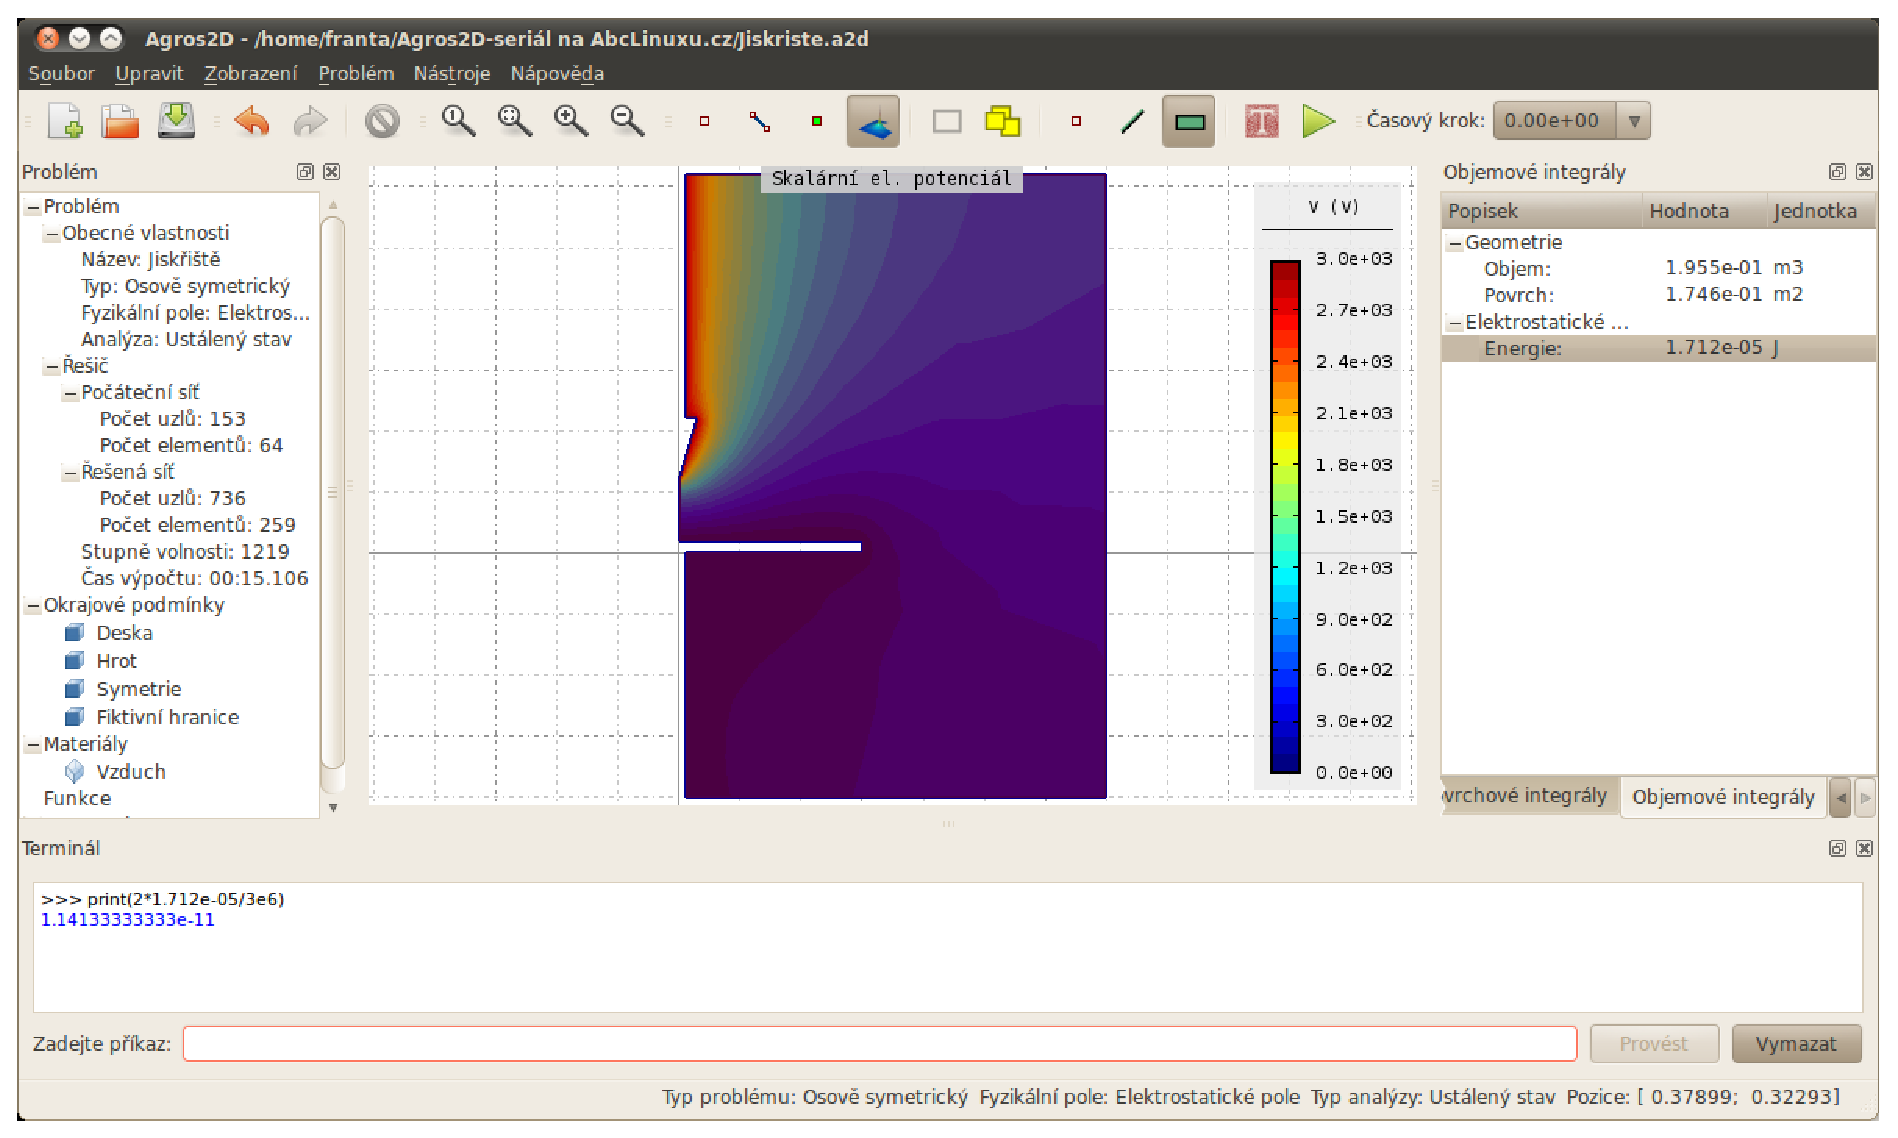
\includegraphics[width=6cm]{Vypocet_kapacity.eps}
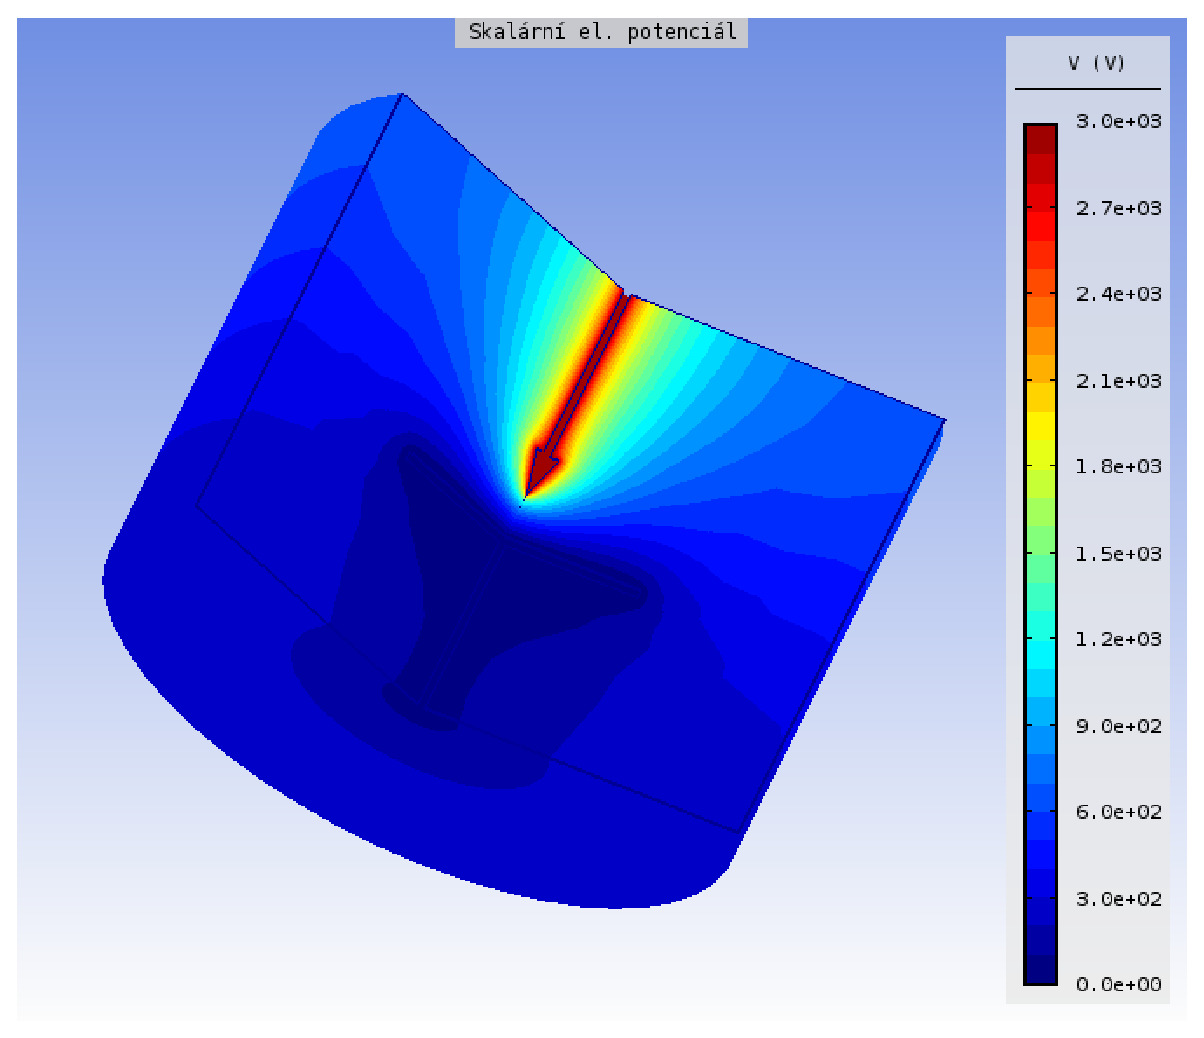
\includegraphics[width=6cm]{Potencial.eps}\\
\subsection{Výpočet indukčnosti dvojlinky}
Při projektování elektrických nebo sdělovacích sítí je velmi důležité znát kromě jiných parametrů také indukčnost použitých kabelů. V tomto příkladě si ukážeme, jak ji vypočítat pro dvojvodičový kabel protékaný stejnosměrným proudem. Budeme tedy řešit magnetostatické pole.\\

\includegraphics[width=6cm]{Matematicky_model_dvojlinky.eps}\\
\subsection{Příprava problému}
Založíme opět nový problém a jako typ řešeného pole zvolíme Magnetické pole, typ problému Kartézský a druh analýzy Ustálený stav. Ostatní nastavení můžeme nechat bez povšimnutí. Agros2D umožňuje kromě standartního ovládání využívat skriptování a také práci pomocí příkazů. Právě práci pomocí příkazů si ukážeme na vytvoření geometrie tohoto příkladu. Všechny funkce a klíčová slova, která můžete při práci využívat naleznete v nápovědě v kapitole Scripting.\\
Mezi základní funkce pro vytváření geometrie patří addnode() (přidání uzlu), addedge() (přidání hrany) a addlabel() (přidání značky oblastí). Vzhledem k podobě geometrie využijeme ale funkci addcircle(), která patří mezi uživatelské a slouží k přidání kružnice, přičemž umožňuje zároveň přiřadit okrajovou podmínku a značku oblasti (materiál).\\
Funkce addcircle() má tři povinné a dva nepovinné parametry. První dva parametry udávají souřadnice středu kružnice a třetí parametr její poloměr. Čtvrtý nepovinný parametr udává, jaká okrajová podmínka se použije na hranici kružnice (pokud není zadána použije se none a hranice bude při řešení uvažována jako rozhraní). Pátý, také nepovinný parametr, značí materiál, který se přiřadí oblasti uvnitř kružnice (pokud se nepoužije nebude značka oblasti do kružnice přiřazena). Je důležité upozornit, že pokud je použit pátý parametr, stává se parametr čtvrtý povinný.\\
Nejprve nadefinujeme okrajové podmínky a materiály, abychom následně mohli plně využít funkci addcircle(). Přidáme jednu okrajovou podmínku, která bude respektovat fiktivní hranici problému a bude jí popisovat Dirrichletova okrajová podmínka. Na této hranici bude vektorový magnetický potenciál roven nule.\\
Při definici materiálů musíme respektovat, že jednotlivými žílami kabelu teče proud vždy opačným směrem. Proto musíme pro jejich definici přidat dva materiály. První z nich (L+) bude mít proudovou hustotu rovnou 2 MA/m2 (tato proudová hustota odpovídá proudu 2 A tekoucího vodičem o průřezu 1 mm2) a druhý (L-) s proudovou hustotou -2 MA/m2. Další materiál, který musíme nadefinovat je izolace kabelu z PVC (Izolace) a jeho okolní prostředí (Prostredi). Izolace kabelu má stejnou permeabilitu jako okolní vzduch a není ji nutné definovat. Pro přehlednost řešeného modelu to však uděláme. Parametry všech materiálů jsou uvedeny v tabulce níže.\\
\begin{tabular}{|c|c|c|c|c|}
\hline
 & L+ & L- & Izolace & Prostředí \\
\hline
Relativní permeabilita & 1 & 1 & 1 & 1\\
\hline
Proudová hustuta & $2 MA/m^2$ & $-2 MA/m^2$ & 0 & 0\\
\hline 
\end{tabular} \\
Nyní již s využitím příkazu addcircle() a postupně vytvoříme celou geometrii.\\
addcircle(-0.000965, 0, 0.000565, "none", "L+")\\
addcircle(0.000965, 0, 0.000565, "none", "L-")\\
addcircle(-0.000965, 0, 0.000965)\\
addcircle(0.000965, 0, 0.000965)\\
addcircle(0, 0, 0.025, "Fiktivni\_hranice")\\
Při přidávání geometrie respektujicí izolaci a okolní prostředí nemůžeme využít automatické přidání značky oblastí, protože ta se vždy přidává do středu kružnice a tak by se značka přidala do nesprávné oblasti. Tyto značky oblasti tedy přidáme ručně nebo můžeme využít příkazu addlabel().\\
addlabel(-0.0002, 0, 0, 0, "Izolace")\\
addlabel(0.0002, 0, 0, 0, "Izolace")\\
addlabel(0, 0.000965, 0, 0, "Prostredi")\\
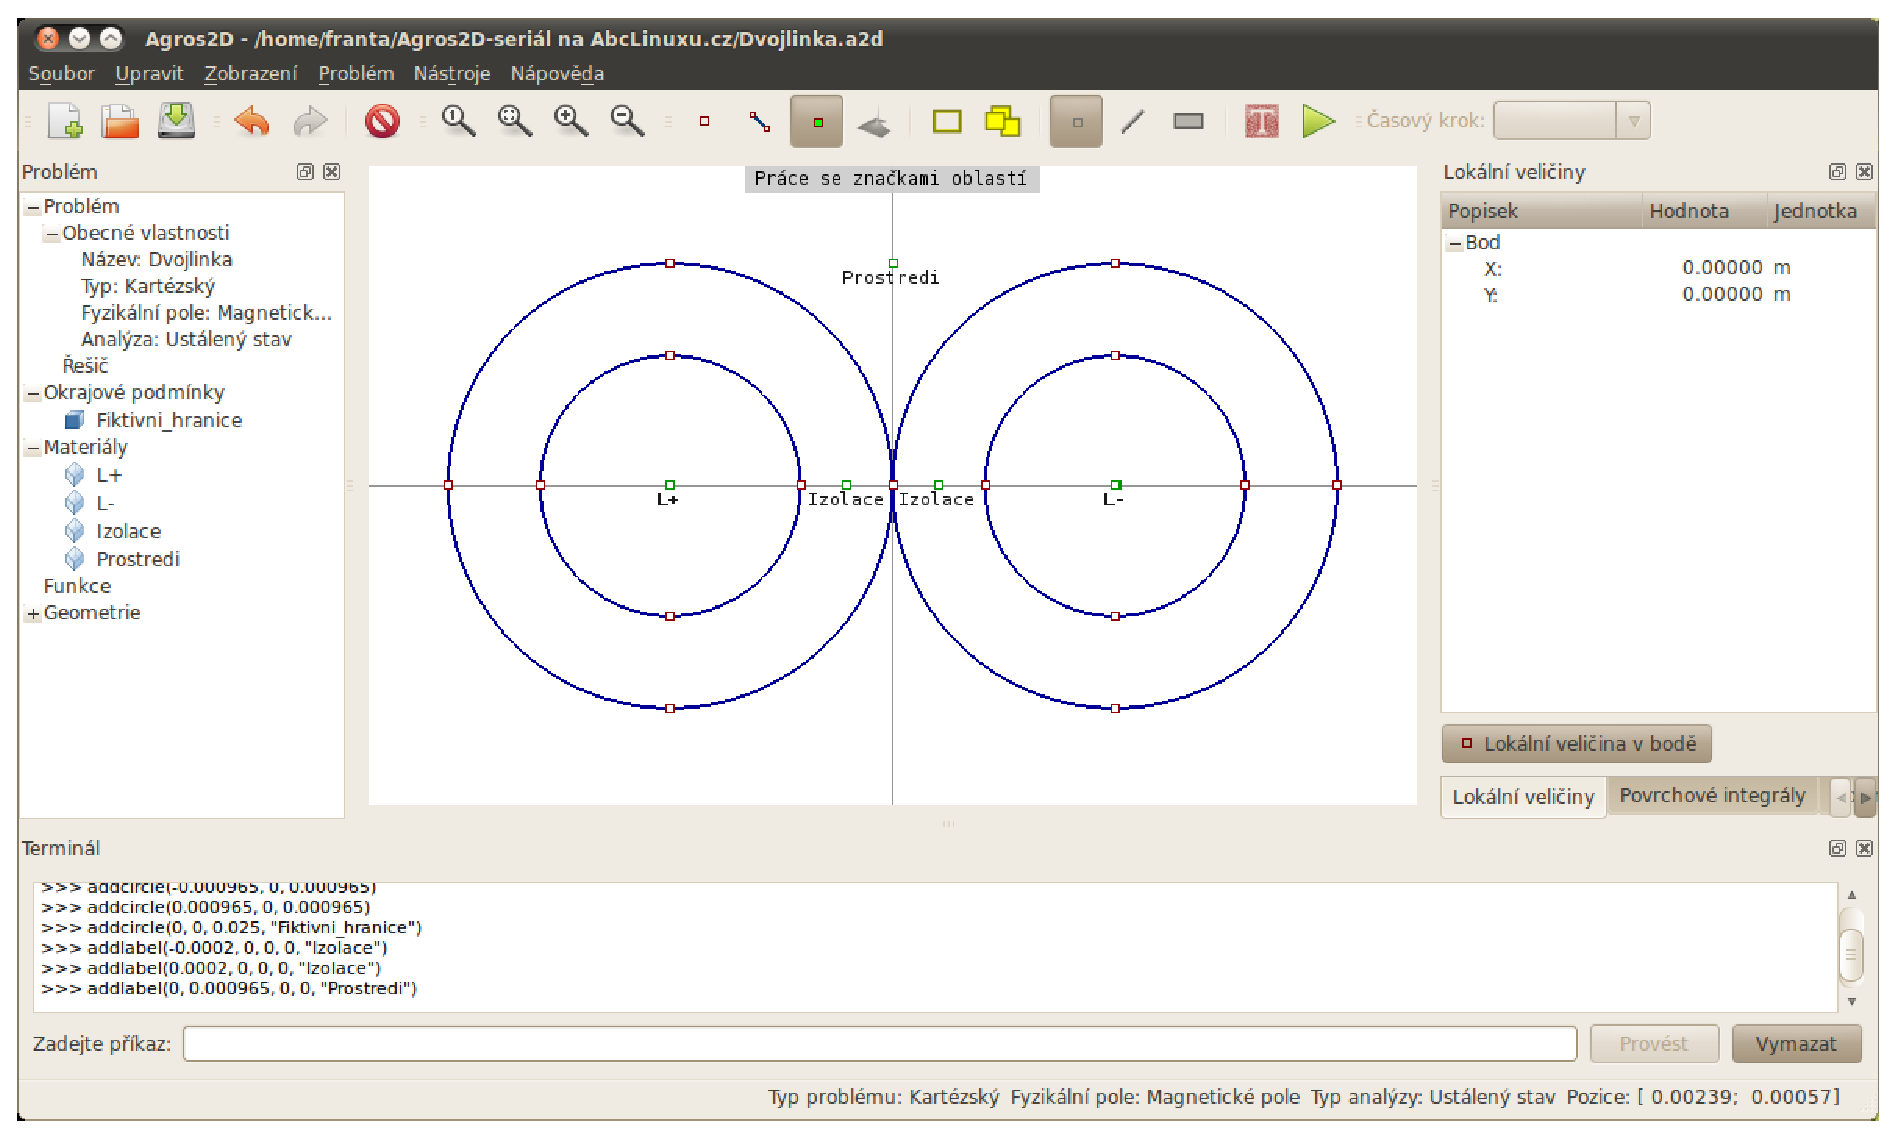
\includegraphics[width=12cm]{Geometrie_druheho_problemu.eps}\\\
\subsection{Řešení}
Při výpočtu budeme postupovat obdobně jako u předchozího příkladu. Pokud diskretizace problému a jeho řešení proběhlo v pořádku, můžeme přistoupit k výpočtu indukčnosti. Opět využijeme energetické definice indukčnosti, kterou lze zapsat do vztahu Wm = $0.5 LI^2$. Nejprve určíme energii magnetického pole ve všech oblastech. Tato energie je rovna $1,185 \mu J$. Pro výpočet využijeme níže uvedený příkaz. Indukčnost dvojlinky je rovna $59,25 \mu H$ na 1 m délky (standardní hloubka u kartézských problému). Pro ilustraci jsou na dalších obrázcích vykresleny siločáry magnetického pole a vektory magnetické indukce.\\
print(2*1.185e-06/2**2)\\
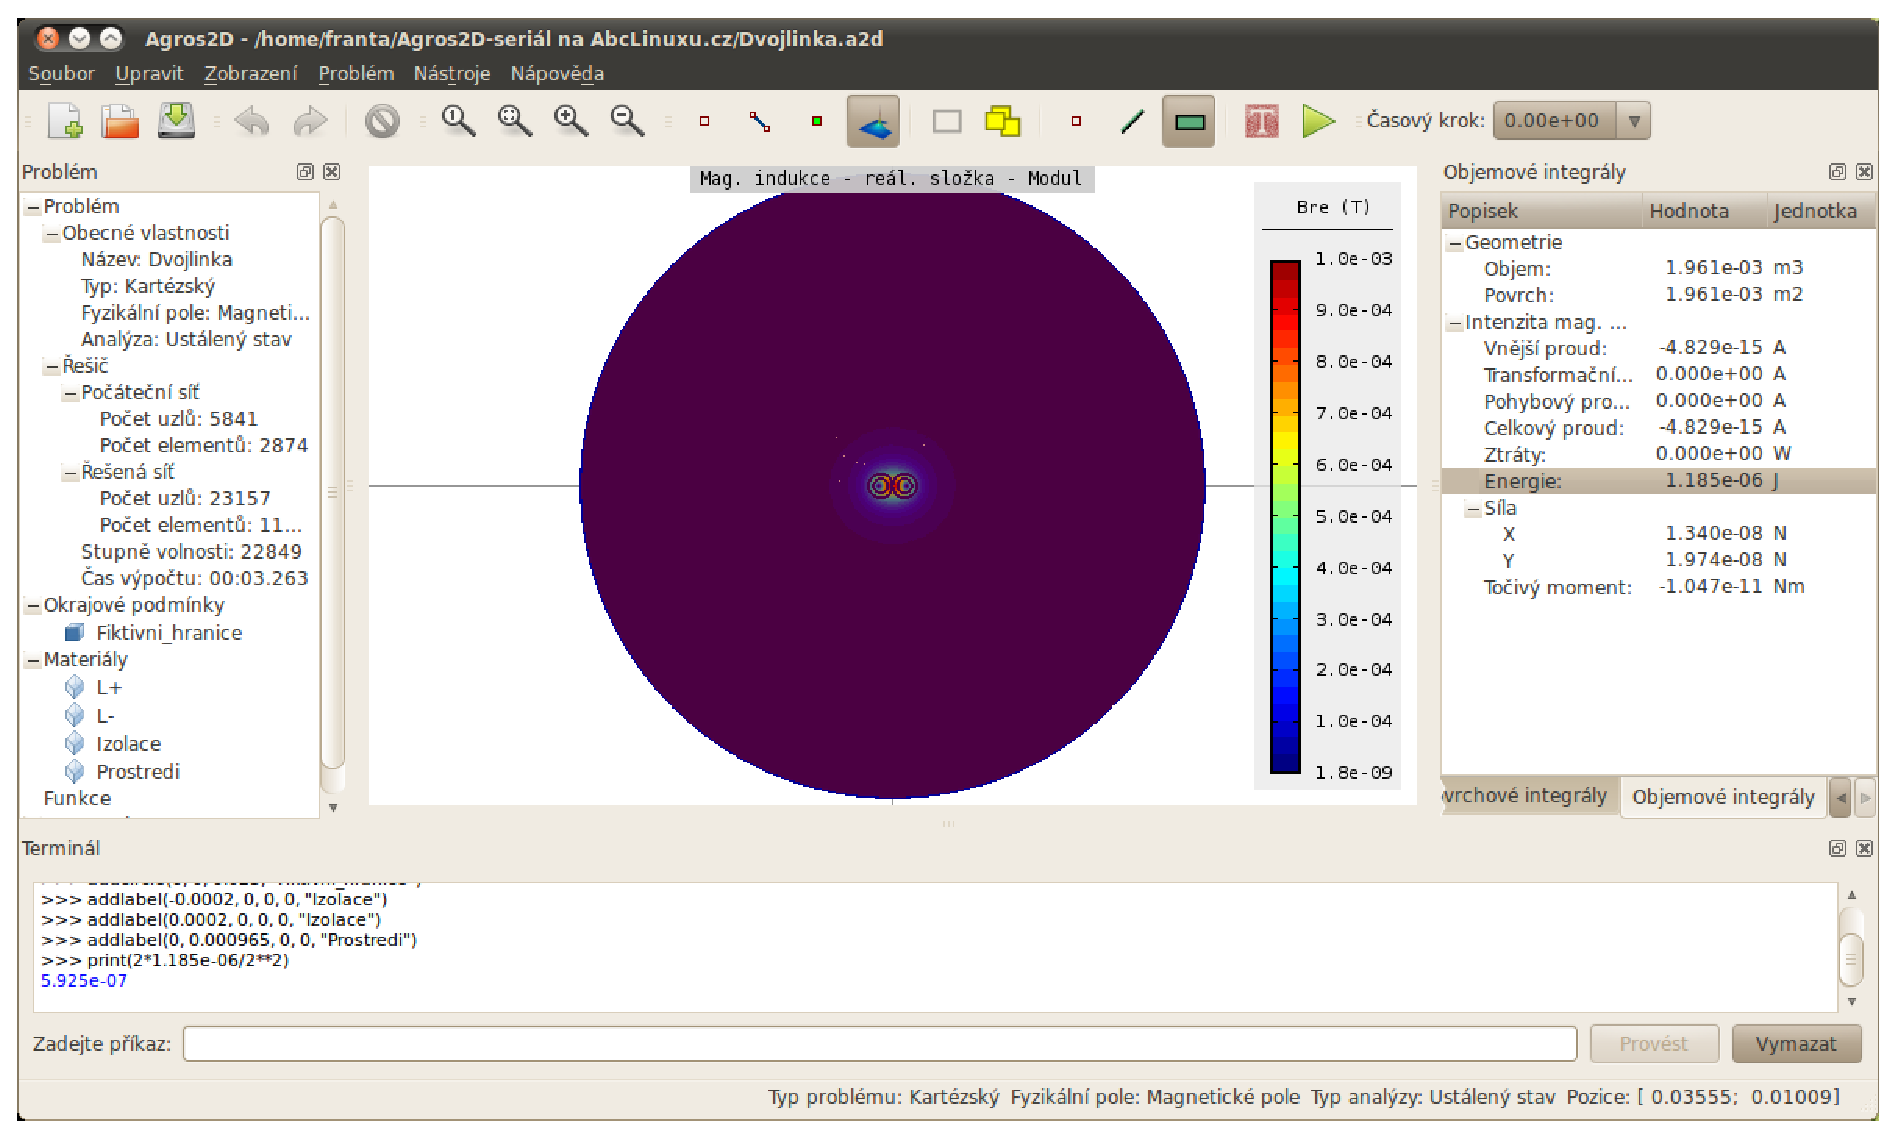
\includegraphics[width=6cm]{Vypocet_indukcnosti.eps}
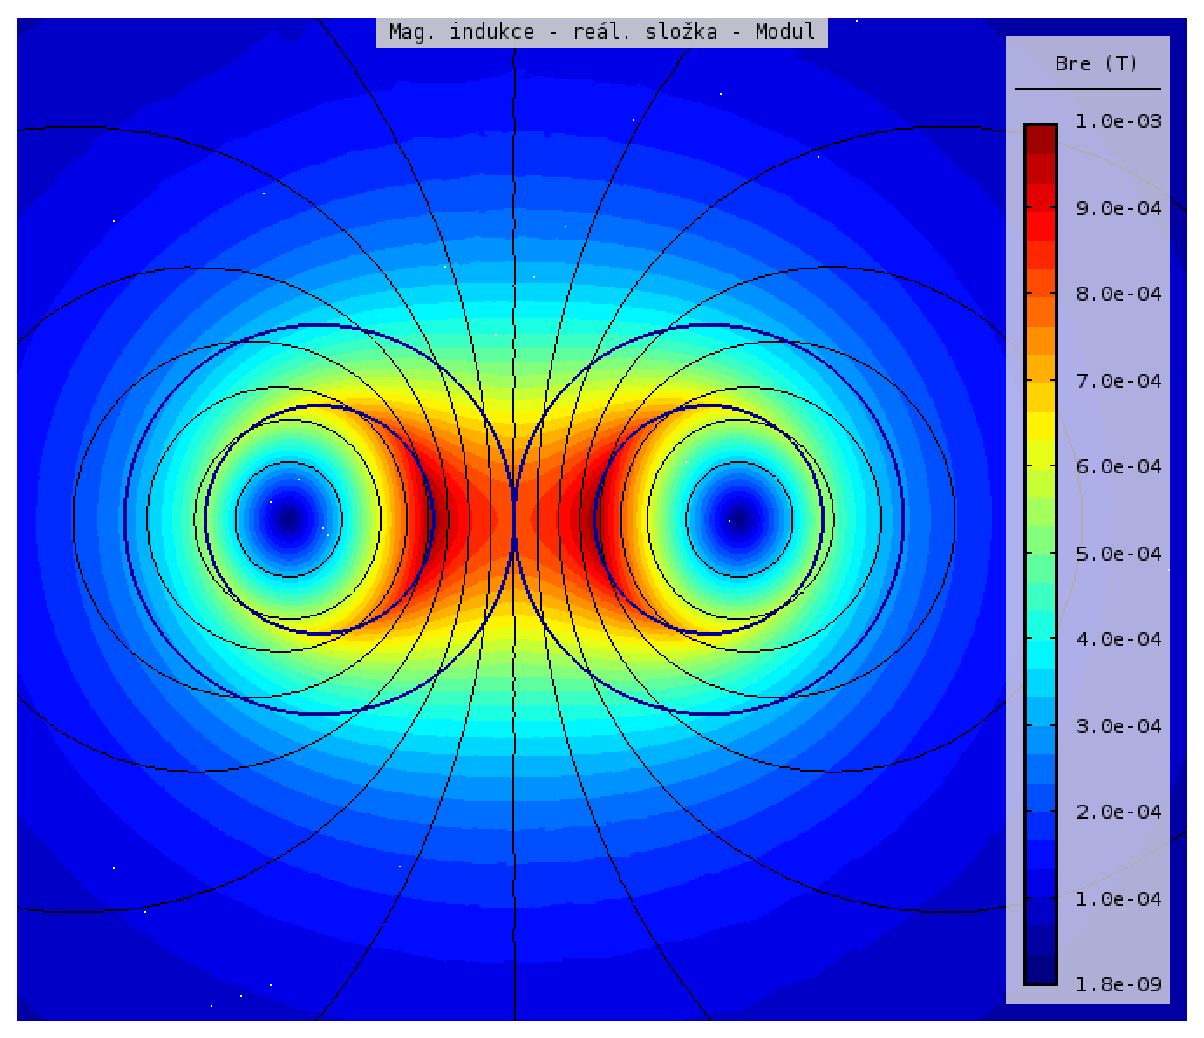
\includegraphics[width=6cm]{Silocary.eps}\\
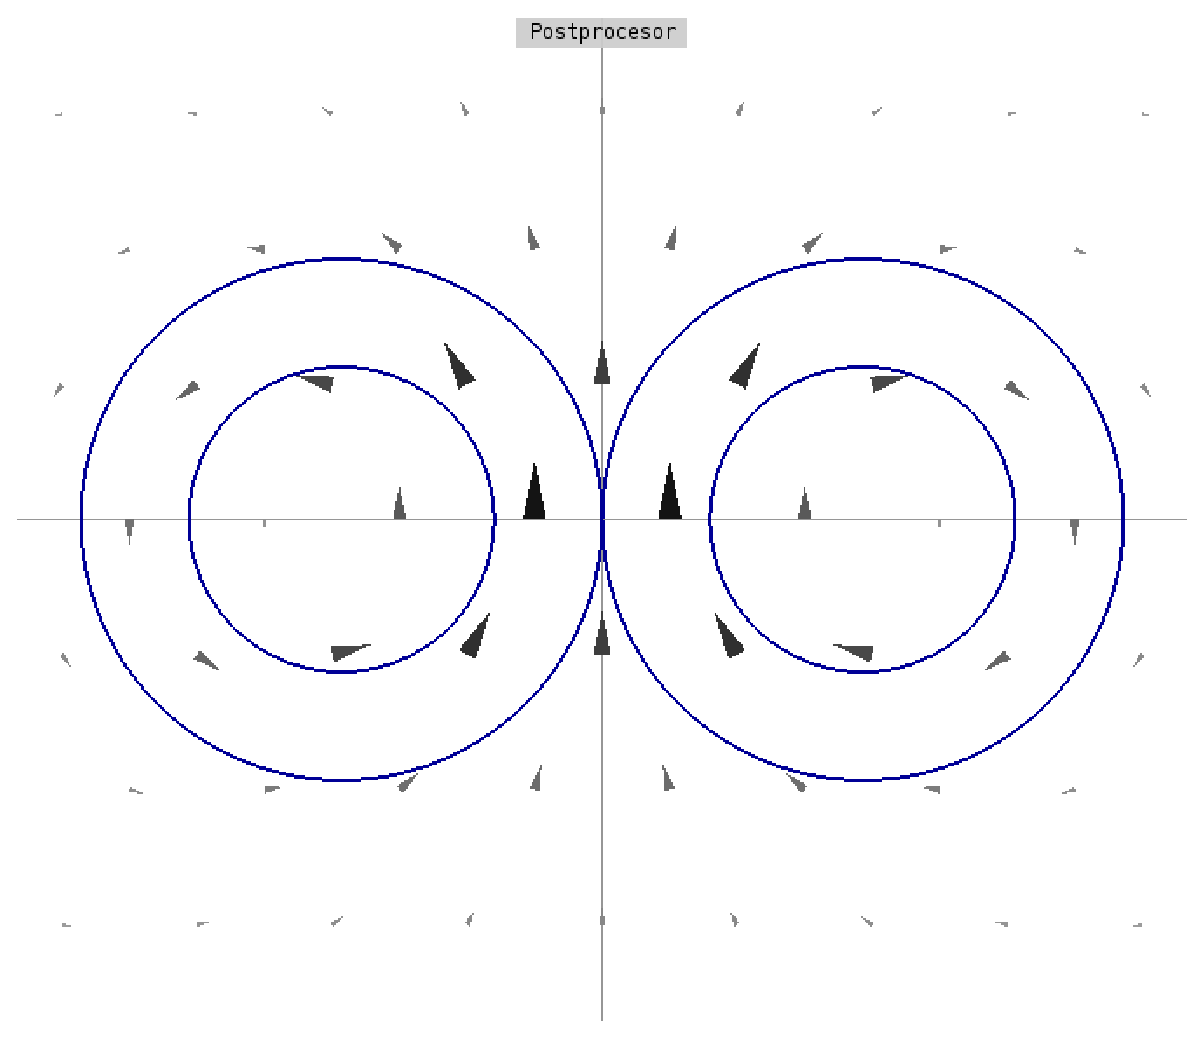
\includegraphics[width=6cm]{Vektory.eps}\\
Příští díl seriálu bude zaměřen především na skriptování a řešení sdružených problémů.\\
\end{document}